% Chapter Template

\chapter{Theoretical Background} % Main chapter title

\label{Chapter2} % Change X to a consecutive number; for referencing this chapter elsewhere, use \ref{ChapterX}

Indoor localization has been a active research field in the last few years. In this chapter the two most common approaches, fingerprinting and range-based, are introduced and their components explained in detail. For the fingerprinting approach I will also talk about \emph{support vector machines} and \emph{the magnetic field in indoor environments}. Although they are not normally used in with fingerprinting they play a vital role in the room recognition system proposed in chapter \ref{Chapter3}. So understanding these concepts will be important.

\section{Range-Based Localization}
\label{therory:range-based}

A range based localization system consists of two main components.

\textbf{A number of Anchor Nodes (ANs)} which are placed at known locations and constantly transmit a radio signal.

\textbf{A mobile node (MN)}, in this case a smartphone, whose location is unknown and needs to be determined.

\begin{figure}[ht]
\centering
\includegraphics[width=\textwidth]{Figures/existingAproach}
\decoRule
\caption[Range-based localization approach]{Block diagram of the range based localization approach.}
\label{fig:existingApproach}
\end{figure}

To determine its position the mobile node measures the received signal strength from each of the anchor nodes $(RSSI_i)$. A ranging model is then used to estimate the distance $(d_i)$ from the mobile node to each anchor node. Because the location of the anchor nodes is known, it is then possible to calculate the position of the mobile node using trilateration. To account for errors during the ranging step the trilateration can also be provided with a set of weights $(w_i)$ representing the accuracy of each distance estimation.

The range-based approach to localization has the benefit of only requiring  a few training samples to train the ranging models. It is therefore easy and not very labour intensive to implement. The problem is that in indoor environments the ranging models are often inaccurate, limiting the localization accuracy that can be achieved with this approach.

In the following subsections the ranging, trilateration and weighting steps are described in further detail.

\subsection{RSSI and signal propagation}

The received signal strength indicator describes the total signal power received in milliwatts with the value expressed on a logarithmic scale (dBm)\cite[p.~160]{sauter2010gsm}. In the case of Wi-Fi a value of -30 would mean a very strong signal while one of -90 would be so low as to be unusable (drowning in noise). In an open space without any obstacles the RSSI mainly depends on the propagation distance, but indoors several other factors become important. These are non line of sight (NLOS) and multipath propagation.

NLOS occurs when the signals path is obstructed by physical objects. The signal has to pass through these objects and therefore the RSSI is lower compared to LOS, where there are no obstacles\cite{JoseMaster}.

Multypath propagation is caused when the signal is reflected from physical objects and arrives at the receiver multiple times with different signal strength. This causes inaccuracy and fluctuations in the measured RSSI as all these signals are blended together\cite{multipathEffects}.

Both of these affects are very common in indoor environments, caused by the walls, people, furniture and other building materials. Furthermore the RSSI values are discrete and not fine grained what causes additional inaccuracy. This makes range-based localization based on RSSI challenging and limits its accuracy.

There are other ways to assess the signal strength, such as channel state information, which is more fine grained and can mitigate multipath effects, but they are not available on most mobile devices\cite{JoseMaster,FineGrainedIndoorTracking}.

\subsection{Ranging}
\label{Ranging}

The ranging process estimates the distance between the ANs and the MN based on the radio parameters, in this case RSSI. This is done with non-linear regression (NLR) and the following model proposed by \cite{li2015passiveWIFIsource}:
\begin{equation} \label{eqn:non-linear path loss model}
d_{i}=\alpha_{i}e^{\beta_{i}RSSI_{i}}
\end{equation}
It describes the loss of signal strength over the propagation distance. \(d_{i}\) is the estimated distance from the MN to the \(i\)-th AN, \(RSSI_{i}\) is the \(i\)-th AN's signal strength as measured by the MN and \(\alpha_{i}, \beta_{i}\) are environment variables specific to each AN.

The model needs to be trained for each AN individually by determining the values for \(\alpha_{i}\) and \(\beta_{i}\). This is done by fitting the function to a small set of training samples. This can be done using, for example, least squares optimization.

\subsection{Trilateration}

Trilateration is the process of determining a absolute or relative location based on the distance to known locations. In contrast to triangulation it relies on distances instead of angles.

In the context of localization the goal is to determine the NM's location \(\left ( x,y \right )\) based on the the locations of the ANs \(\left ( \tilde{x_{i}},\tilde{y_{i}} \right )\) and the distance estimations \(d_{i}\) obtained from the path loss model.

The actual distance \(D_{i}\) from the MN to the \(i\)-th AN can be expressed as follows:
\begin{equation}
D_{i} = \sqrt{\left ( \tilde{x_{i}}-x \right )^{2}+\left ( \tilde{y_{i}}-y \right )^{2}}
\label{eqn: distance MN to AN_{i}}
\end{equation}
Under the assumption that \(d_{i}=D_{i}\)  this leads to the following equation system:
\begin{equation}
\begin{pmatrix}
d_{1}\\ 
d_{2}\\
\vdots\\
d_{n}
\end{pmatrix}
=
\begin{pmatrix}
\sqrt{\left ( \tilde{x_{1}}-x \right )^{2}+\left ( \tilde{y_{1}}-y \right )^{2}}\\
\sqrt{\left ( \tilde{x_{2}}-x \right )^{2}+\left ( \tilde{y_{2}}-y \right )^{2}} \\
\vdots\\
\sqrt{\left ( \tilde{x_{n}}-x \right )^{2}+\left ( \tilde{y_{n}}-y \right )^{2}}
\end{pmatrix}
\label{eqn: trilateration problem as equation system}
\end{equation}

But \(d_{i}\) is only an estimation so there is no exact solution of the above system. The best solution is the one that minimizes the sum of the squared error \(d_{i} - D_{i}\). So to determine the MN's location the following problem has to be solved:
\begin{equation}
argmin_{x,y}\sum_{i=1}^{n}w_{i}\left ( d_{i} - \sqrt{\left ( \tilde{x_{i}}-x \right )^{2}+\left ( \tilde{y_{i}}-y \right )^{2}} \right )^{2}
\label{eqn: trilateration as optimization problem}
\end{equation}
This can be done using a optimization algorithm like "Levenberg–Marquardt" or "Gauss-Newton".

\subsection{Weighting}

The optimization problem in equation \ref{eqn: trilateration as optimization problem} also defines a set of weights $w_i$ coresponding to each distance estimation $d_i$. In the context of trilateration these weights represent how accurate each distance estimation is.

The ranging models accuracy can vary greatly. By applying a large weight to the more accurate estimations and a small weight to the inaccurate ones it should, in theory, be possible to correct for the ranging error and improve the localization.

In practice the problem is, that the ranging error is not known. A weighting method is needed that estimates the ranging error.

Previous work at the CDS group \cite{FineGrainedIndoorTracking} used the assumption that the ranging error is larger with increasing distance to the anchor node. So the weights were defined as inversely proportional to the estimated distances:

\begin{equation}
w_{i}=\frac{{d_i}^{-1}}{\sum_{n=1}^{N}{d_n}^{-1}}
\label{eqn: distance weights}
\end{equation}

\section{Fingerprinting}

Fingerprinting is a common method for localization based on RSSI\cite{chapre2013RSSI}. It consists of two main phases.

In the offline/training phase a map of reference points (RP) is created by collecting RSSI values for each AN from known locations.
Then in the online phase RSSI values are collected from an unknown location, called the test point (TP). The location of the TP is determined based on the RP-map using machine learning algorithms like  a k-nearest neighbor regression\cite{JoseMaster}.

The accuracy of this method mainly depends on the density of the RP-map. The higher the density of RPs the better the accuracy. Generally achieving a satisfying level of accuracy, requires a lot of RPs. Other factors are the number of attributes in each RP and the variability of the observation parameters.

More attributes per RP, an attribute being a data value like a RSSI or a magnetic field measurement, gives the algorithm more information to work with and so increased the accuracy\cite{Li2012feasableMagnetic}. This effect is subject to diminishing returns\cite{brouwers2014incremental}. A high variability in the observation parameters depending on location is also beneficial.

This approach is able to achieve good accuracies in an indoor environment. The problem is that it is very labour intensive to create the necessary fingerprinting maps.

\subsection{Magnetic field in indoor environments}

Earths natural magnetic field has already been used for localization, mainly as a compass to determine the devices heading in PDR systems. However, the presence of magnetic field anomalies make accurate heading determination difficult for indoor applications. The anomalies are caused by the ferrous structures in the building materials, electrical devices, cables and tubes. Previous research suggests that these anomalies can be used in a fingerprinting approach to determine a devices location\cite{haverinen2009global,angermann2012CharacterizationMagnetic,Li2012feasableMagnetic}. They show that the magnetic field anomalies have sufficient local variability and are mostly stable over time. Therefore they should be applicable for use in localization.

\subsection{Support Vector Machine}
\label{theory:SVM}
The Support Vector Machine (SVM) is one of the most widely used machine learning algorithms. It predicts the labels of new (unknown) samples based on previous (known) examples. In its basic form it only supports two labels. This is called binary classification.

The known examples are called training data. It consists of instance-label pairs \(\left ( x_{i}, y_{i} \right ), i=1,...,l\) where \(x_{i}\in R^{n}\) and \(y_{i}\in \left \{ -1,1 \right \}\). \(x_{i}\) represents the samples's observable features while the label \(y_{i}\) defines in which category it belongs.

The SVM maps the samples into \(n\)-dimentional space and then tries to fit a hyperplane through that space separating the two classes so that ideally all samples with \(y_{i}=1\) are on one side of the hyperplane and \(y_{i}=-1\) on the other. To make the separation as clear as possible the margin between the hyperplane and the samples is maximized at the same time. The samples which lie directly on the margins are called the support vectors.

To classify a new unknown sample the SVM determines on which side of the hyperplane it lies and assigns the according label.

To fit the hyperpalane the SVM solves the following optimization problem\cite{chang2011libsvm}:
\begin{equation}
\begin{split}
\min_{\omega , b ,\xi}\;\; & \frac{1}{2}\omega^{T}\omega +C\sum_{i=1}^{l}\xi_{i}\\
\textup{subject to}\;\; & y_{i}\left ( \omega^{T}\phi \left ( x_{i} \right )+b \right )\geq 1-\xi_{i},\\
& \xi_{i}\geq 0,i=1,...,l
\end{split}
\end{equation}

There may be outlines in the data, so a hyperplane that separates all samples correctly may not be the best classifier. To account for this, a cost is paid if a sample violates the error term \(y_{i}\left ( w^{T}\phi \left ( x_{i} \right )+b \right )\geq 1\), increasing the objective function by \(C \xi_{i}\). The $C$ parameter defines the trade-off between the simplicity of the decision surface (\emph{hyperplane}) and misclassification of training samples. For large values of $C$ the optimization will chose a hyperplane with a smaller margin, more support vectors and therefore more complex decision surface, trying to classify all samples correctly. Conversely, a small value of $C$ will cause the optimizer to look for a larger-margin separating hyperplane, even if that hyperplane misclassifies some samples\cite{crossValidatedSVMC}.

\begin{figure}[htp]

\label{fig:SVM}
\centering
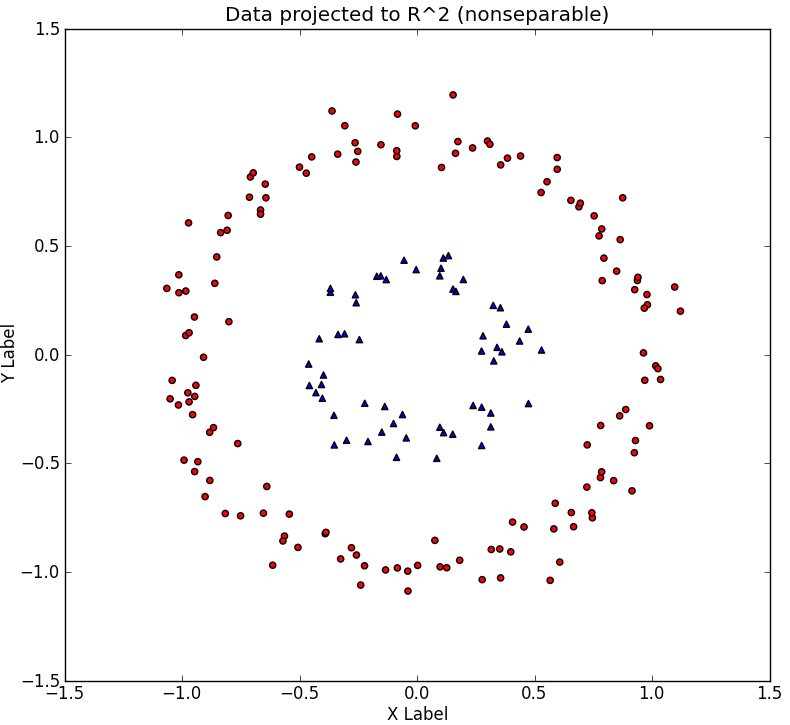
\includegraphics[width=.3\textwidth]{Figures/svm_1.png}\hfill
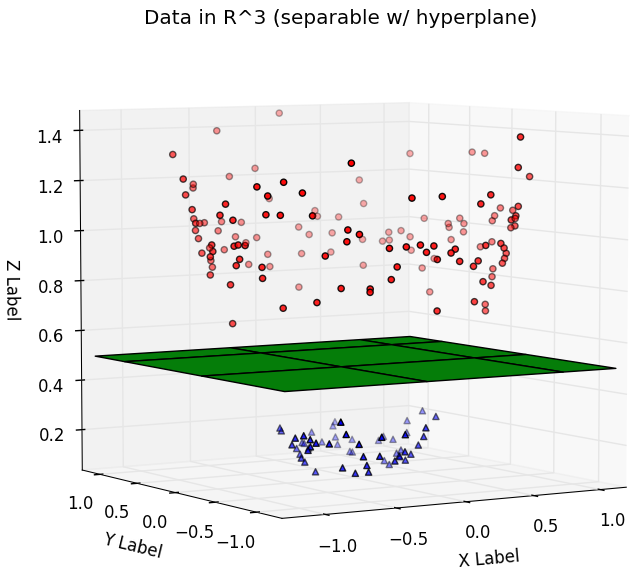
\includegraphics[width=.3\textwidth]{Figures/svm_2.png}\hfill
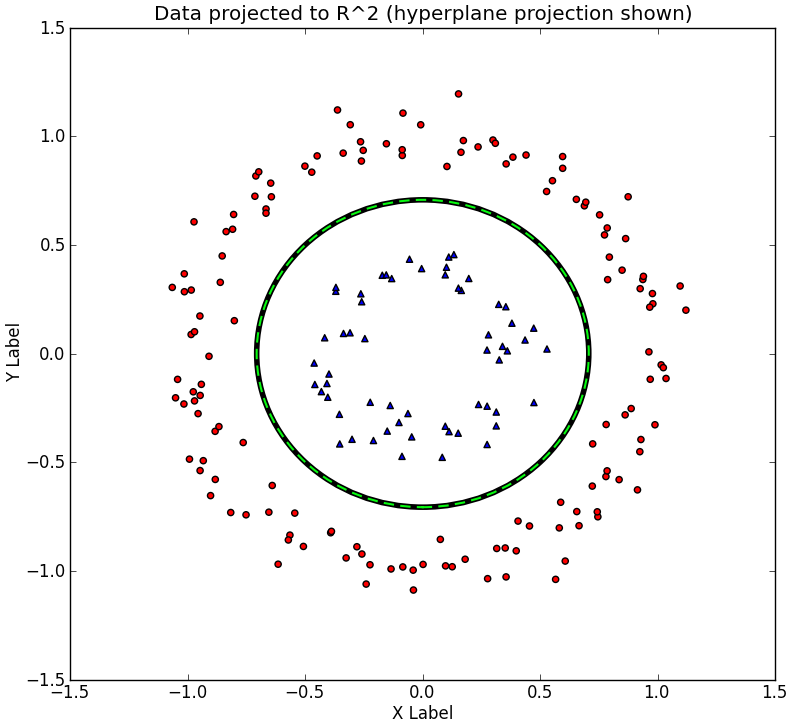
\includegraphics[width=.3\textwidth]{Figures/svm_3.png}
\decoRule
\caption[SVM kernel trick]{\raggedright(Left) A dataset in, not linearly separable. (Middle)The same dataset transformed with decision boundary. (Right) The nonlinear decision boundary.}

\end{figure}

But the training data may not be linearly separable. In this case the so called kernel trick can be used. The kernel is a function \(k\left ( x_{i}, x_{j} \right )=\phi \left ( x_{i} \right )\cdot \phi\left ( x_{j} \right )\) which maps the features \(x_{i}\) to a higher dimensional space where they can be separated by a hyperplane. This results in a non linear separation in the original feature space\cite{ErikKimKernelTrick}.

To perform multy-class classification the "one-against-one" approach can be used. For \(k\) classes \(k\left ( k-1 \right )/2\) classifiers are trained. Each binary classifier is then considered to vote for a class. The sample is then placed in the class with the most votes\cite{chang2011libsvm}.